\documentclass[bachelor, och, coursework, times]{SCWorks}
% параметр - тип обучения - одно из значений:
%    spec     - специальность
%    bachelor - бакалавриат (по умолчанию)
%    master   - магистратура
% параметр - форма обучения - одно из значений:
%    och   - очное (по умолчанию)
%    zaoch - заочное
% параметр - тип работы - одно из значений:
%    referat    - реферат
%    coursework - курсовая работа (по умолчанию)
%    diploma    - дипломная работа
%    pract      - отчет по практике
%    pract      - отчет о научно-исследовательской работе
%    autoref    - автореферат выпускной работы
%    assignment - задание на выпускную квалификационную работу
%    review     - отзыв руководителя
%    critique   - рецензия на выпускную работу
% параметр - включение шрифта
%    times    - включение шрифта Times New Roman (если установлен)
%               по умолчанию выключен 
%убирание преносов слов
\tolerance = 1
\emergencystretch = \maxdimen
\hbadness = 10000


\usepackage[colorlinks=false, pdfborder={0 0 0}]{hyperref}  % убирает и цвет, и рамки
\usepackage[T2A]{fontenc}
\usepackage[utf8]{inputenc}
\usepackage[english,russian]{babel}
\usepackage{graphicx}
\usepackage[sort,compress]{cite}
\usepackage{amsmath}
\usepackage{amssymb}
\usepackage{amsthm}
\usepackage{fancyvrb}
\usepackage{longtable}
\usepackage{array}
\usepackage{minted}
\usepackage{tempora}
\usepackage{listings}
\usepackage{verbatim}



\newcommand{\eqdef}{\stackrel {\rm def}{=}}
\newcommand{\No}{\textnumero}
\newtheorem{lem}{Лемма}
\setminted{style=bw,
	linenos=true,
	breaklines=true,
	numbersep=5pt,
	tabsize=2,
	fontsize=\small,
	bgcolor=white}
\setmintedinline{style=bw,
	bgcolor=white,
	fontsize=\normalsize
	}
\begin{document}
    
   % Кафедра (в родительном падеже)
    %\chair{математической кибернетики и компьютерных наук}
    \chair{математической кибернетики и компьютерных наук}
    % Тема работы
    \title{Разработка базового функционала для обучающей компьютерной ролевой игры}
    
    % Курс
    \course{2}
    
    % Группа
    \group{211}
    
    % Факультет (в родительном падеже) (по умолчанию "факультета КНиИТ")
    \department{факультета компьютерных наук и информационных технологий}
    
    % Специальность/направление код - наименование
    
    \napravlenie{02.03.02 "--- Фундаментальная информатика и информационные технологии}
    
    % Для студентки. Для работы студента следующая команда не нужна.
    \studenttitle{студентки}
    
    % Фамилия, имя, отчество в родительном падеже
    \author{Никитенко Яны Валерьевны}

    % Заведующий кафедрой
\chtitle{доцент, к. ф.-м. н.} % степень, звание
\chname{С.\,В.\,Миронов}

%Научный руководитель (для реферата преподаватель проверяющий работу)
\satitle{доцент, к.т.н.} %должность, степень, звание
\saname{М.\,В.\,Хамутова}

% Руководитель практики от организации (только для практики,
% для остальных типов работ не используется)
%\patitle{доцент, к. ф.-м. н.} 
%\paname{М.\,И.\,Сафрончик}

% Семестр (только для практики, для остальных
% типов работ не используется)
\term{3}

% Наименование практики (только для практики, для остальных
% типов работ не используется)
\practtype{учебная}

% Семестр (только для практики, для остальных
% типов работ не используетс
    
    % Заведующий кафедрой 
    %\chtitle{доцент, к.\,ф.-м.\,н.}
    %\chname{С.\,В.\,Миронов}
    % Научный руководитель (для реферата преподаватель проверяющий работу)
    %\satitle{доцент, к.\,ф.-м.\,н.} %должность, степень, звание
    %\saname{А.\,П.\,Грецова}
    % Руководитель ДПП ПП для цифровой кафедры (перекрывает заведующего кафедры)
    % \chpretitle{
    %     заведующий кафедрой математических основ информатики и олимпиадного\\
    %     программирования на базе МАОУ <<Ф"=Т лицей №1>>
    % }
    % \chtitle{г. Саратов, к.\,ф.-м.\,н., доцент}
    % \chname{Кондратова\, Ю.\,Н.}
    \date{2025}
    
    
    % Руководитель практики от организации (руководитель для цифровой кафедры)
    %\patitle{доцент, к.\,ф.-м.\,н.}
    %\paname{С.\,В.\,Миронов}
    
    % Руководитель НИР
    %\nirtitle{доцент, к.\,п.\,н.} % степень, звание
    %\nirname{В.\,А.\,Векслер}
    
    % Семестр (только для практики, для остальных типов работ не используется)
    %\term{2}
    
    % Наименование практики (только для практики, для остальных типов работ не
    % используется)
    %\practtype{учебная}
    
    % Продолжительность практики (количество недель) (только для практики, для
    % остальных типов работ не используется)
    \duration{18}
    
    % Даты начала и окончания практики (только для практики, для остальных типов
    % работ не используется)
    \practStart{02.09.2024}
    \practFinish{12.01.2025 }
    
    % Год выполнения отчета
   
    
    \maketitle

    % Включение нумерации рисунков, формул и таблиц по разделам
    % (по умолчанию - нумерация сквозная)
    % (допускается оба вида нумерации)
    %\secNumbering

    
    
    \tableofcontents
    
    % Раздел "Обозначения и сокращения". Может отсутствовать в работе
    %\abbreviations
    %\begin{description}
    %    \item $|A|$  "--- количество элементов в конечном множестве $A$;
    %    \item $\det B$  "--- определитель матрицы $B$;
    %    \item ИНС "--- Искусственная нейронная сеть;
    %    \item FANN "--- Feedforward Artifitial Neural Network
    %\end{description}
    
    % Раздел "Определения". Может отсутствовать в работе
    %\definitions
    
    % Раздел "Определения, обозначения и сокращения". Может отсутствовать в работе.
    % Если присутствует, то заменяет собой разделы "Обозначения и сокращения" и "Определения"
    %\defabbr
    
    
    % Раздел "Введение"
    \intro
    Целью курсового проекта является разработка базового функционала 
    для компьютерной игры используя Unity. Реализация таких задач как:
    \begin{itemize}
     
\item  Передвижения персонажа
\item Инвентарь(добавление предметов, проверка на заполненность инвентаря)
\item Система цепочки заданий
\item Боевая Система
\item Диалоговая система
\end{itemize}

Проект является игровым приложением в жанре RPG(анг.Role-playing game).
Основу игрового процесса составляет выполнения различных заданий(в первую очередь
главного сюжетного задания),развития навыков и характеристик в ходе сражений
и использования навыков. При желании разработчик может добавлять другие 
дополнительные механики(к примеру ремесло), которые помогут выделить игру
на фоне конкурентов. 

В данной курсовой работе будет разработаны базовые функции для игры,
которые выше перечислены были.

\section{Анализ предметной области разработки компьютерных игр}

    В самом общем смысле, компьютерную игру можно определить как интерактивную программную систему,
     в которой один или несколько игроков, воздействуя через устройства ввода 
     (клавиатура, мышь, джойстик, сенсорный экран и т.д.), 
     управляют виртуальными объектами (персонажами, процессами, средами)
      в рамках заданных правил с целью достижения определенных результатов, 
      часто связанных с вызовом, развлечением, обучением или социальным взаимодействием.


    \subsection{Постановка задачи разработки игры 
    (Актуальность, цель, назначение и описание целевой аудитории )}

    Славянская мифология, является богатейшим пластом культурного наследия Восточной Европы, 
    остается значительно менее представленной в массовой игровой индустрии 
    по сравнению с скандинавской, греческой или кельтской мифологиями. 
    Существует растущий спрос со стороны аудитории 
    на аутентичные и глубокие погружения в это самобытное мифологическое пространство.

    Несмотря на наличие некоторых игр, затрагивающих славянскую тематику, 
    ощущается дефицит полноценных РПГ, целостно и уважительно раскрывающих мир славянских духов, 
    божеств, обрядов и эпических сказаний. Большинство проектов либо поверхностны, 
    либо используют мифологию лишь как декоративный фон.

    В этой игре в центре сюжета оказываются именно мифические создания, их проблемы,
    взгляд на мир людей и непосредственно конфликт с ним.

    Собственно цель проекта популяризировать славянский фольклор и культуру, в особенности
    среди молодого поколения. Т.е основной целевой аудиторией являются
    люди от 14 до 30 лет. 


    \subsection{Исследование понятия и классификация компьютерных игр}

    Из-за огромного разнообразия игр, их целей, механик и платформ, создание единой, 
    всеобъемлющей классификации является сложной задачей. 
    Классификации часто пересекаются и дополняют друг друга. 
    Как правило классифицировать игры можно по:

      \begin{enumerate}
     
\item Жанру
\item Платформе
\item Количеству игроков и режиму взаимодействия
\item Модели монетизации
\item Целевому назначению и содержанию

\end{enumerate}


    \subsection{Обоснование и обзор выбранного жанра игры}
    
    Компьютерная ролевая игра (англ. computer role-playing game, 
    обозначается аббревиатурой CRPG или RPG) — жанр компьютерных игр, 
    в котором игрок управляет одним или несколькими персонажами, 
    каждый из которых описан набором численных характеристик, 
    списком способностей и умений; примерами таких характеристик могут быть очки здоровья 
    (англ. hit points, HP), показатели силы, ловкости, интеллекта, защиты, уклонения,
     уровень развития того или иного навыка и т. п.\cite{gamedes}

    Данный жанр был выбран по следующим причинам:

\begin{itemize}
     
\item Личная мотивация - автор давно знаком с этим жанром, хорошо знаком с механиками
и искренне любит его
\item Зачастую игры вдохновленные мифами выпускаются в этом жанре
\end{itemize}

    \subsection{Описание геймплея разрабатываемой игры}

    Основой геймплея является: выполнение заданий(убийства монстров, сбор предметов,
    защита и сопровождение NPC, разведка, разговор с NPC(Non-player character) и т.д), развития персонажа
    (повышение характеристик, улучшение и получение новых навыков), 
    исследование мира, занесение в кодекс информации о мире.

    В этом проекте, будет реализовано пока только выполнения заданий со сбором и убийством монстров.
    А так же кодекс, в прологе будет одна запись о существе "Жар-птица" на начало игры,
    что-бы игрок больше узнал за кого он будет играть. 
    Далее заполнение кодекса должно будет стать частью игрового процесса.
    Заполнение кодекса будет происходить, во время путешествий по миру игры.
    

    В дальнейшем в развитии проекта все элементы будут получать развитие.

    В данной курсовой работе будет реализован только пролог с базовыми и простыми механиками,
    которые познакомят с тем, что его будет ждать в дальнейшем.

    В основном информация для кодекса берется из книги 
    "Славянские мифы от Велеса и Мокоши до Птицы Сирин и Ивана Купалы" автора А. Л Барков.\cite{slavick}


    \subsection{Обоснование и выбор инструментов создания игры 
    (анализ игровых движков, графических 
    редакторов и других инструментов разработки игры)}

    На данный момент времени существует множество инструментариев для
    облегчения процесса создания видеоигр. Одним из таких являются движки, 
    редакторы кода и другие.

    На данный момент все ныне существующие игровые движки используют параллельные вычисления, 
    однако не во всех аспектах – так, 
    например многопоточной обработке подвергаются рендеринг изображения, 
    обработка физических вычислений, обработка звуковых дорожек. 
    Несмотря на это, логика игры, ее правила и механики обрабатываются в одном потоке 
    одного ядра ЦП, что, 
    при большом масштабе проекта выливается в так называемые “фризы” – моменты, 
    когда в очереди на выполнение оказывается множество команд и 
    время обработки значительно вырастает.

Решить данную проблему призван архитектурный паттерн 
Entity – Component – System (ECS), 
который заменяет традиционную для разработки игр парадигму 
объектно-ориентированного программирования 
на параллельное программирование и работу с данными.

Был проведен анализ следующих игровых движков.

 \begin{itemize}
     
\item  Unity

Unity является одним из популярных движков, 
использующий язык программирования C\#. 
Данный продукт предоставляет множество платных и бесплатных асетов, 
которые помогут разработчикам в создании игры. 
Также существует пробная версия дополнительных программных пакетов D.O.T.S., 
позволяющая применять параллельные вычисления ко всем игровым составляющим 
— логика, физика, видео- и звуковые потоки.

В Unity используется среда .NET и язык программирования C\# — самый популярный в разработке игр. 
Движок компилирует код C\# для каждого целевого устройства, 
поэтому вы можете развертывать приложения для ПК, мобильных устройств, консолей,
 а также платформ AR и VR.\cite{search1}

\item Unreal Engine 4

Unreal Engine универсальный и очень гибкий движок, 
использующий язык программирования C++. 
Он наполнен множеством бесплатных инструментов разработки. 

В версии 4 компания Epic Games сделала упор на простоту пользования.

В соответствии с фокусом UE4 на простоте, 
он включает новую визуальную систему сценариев под названием «Blueprints» 
(преемник «Kismet» UE3), которая позволяет быстро разрабатывать игровую логику 
без использования кода, что приводит к уменьшению разрыва между техническими художниками, 
дизайнерами и программистами.\cite{search2}

Его преимуществом является поддержка UltraHD разрешения графики и прямая работа 
с памятью с помощью встроенных библиотек. 
Параллельные вычисления можно осуществлять с помощью встроенного в C++ 
планировщика задач, однако его невозможно применить к чему-либо, 
кроме логической части игры и физическим вычислениям.

\item CryEngine

CryEngine на данный момент представляет разработчикам возможность делать 
в своих проектах фотореалистичную графику.\cite{search3} 
Данный движок предоставляет встроенную поддержку мультипотопных вычислений, 
однако, так же, как и в Unreal Engine, 
они применимы лишь на логическую и физическую части игрового проекта. 

Движок использует язык программирование C++.


\item Godot

Godot развивающийся движок, использующий собственный язык программирования - GDScript. 
Присутствует поддержка C++ и C\#, в скором времени и Python. 
Идеально подойдет для знакомства с разработкой игр, 
если у пользователя уже есть небольшой опыт в программировании. 
Также имеет встроенный функционал распараллеливания процессов 
с помощью планировщика задач. 

Узлы организованы внутри «сцен», которые являются повторно используемыми, инстанцируемыми, 
наследуемыми и вложенными группами узлов. Узлы соединены сигналами, 
которые могут передавать объекты данных. Все игровые ресурсы, включая скрипты и графические активы, 
сохраняются как часть файловой системы компьютера (а не в базе данных ). 
Это решение для хранения предназначено для облегчения совместной работы 
между командами разработчиков игр, использующими системы контроля версий программного обеспечения.\cite{search4}

\item GameMaker Studio

GameMaker Studio — один из самых известных игровых движков 
наравне с Unity и Unreal Engine.
 На нем сделаны многие инди-хиты вроде Undertale,
  а еще у него очень низкий порог вхождения: 
  для GameMaker необязательно умение программировать, 
  и все взаимодействия можно настраивать буквально «перетягиванием».

GameMaker позволяет создавать кроссплатформенные и многожанровые видеоигры 
с использованием пользовательского визуального языка программирования 
с функцией перетаскивания или языка сценариев , известного как Game Maker Language (GML), 
который можно использовать для разработки более сложных игр. 
GameMaker изначально был разработан, 
чтобы позволить начинающим программистам создавать компьютерные игры без особых знаний 
в области программирования, используя эти действия. 
Последние версии программного обеспечения также ориентированы на продвинутых разработчиков.\cite{gamemakerstudio}
 \end{itemize}

\section{Описание разработки игры}

    Для разработки игры используются: функционал движка Unity, версия 6000.0.32f1, 
    язык программирования C\#, редактор кода Microsoft Visual Studio Community 2022 
    (64-разрядная версия) - Current версия 17.4.4, растровый графический редактор Krita версия 5.2.2
    и редактор изображений Aceprite версия v1.3.14.2.

    В самом начале проекта был нарисован спрайт персонажа, которым 
    будет управлять игрок и портрет персонажа в меню. Ниже представлены этапы рисования портрета
    в Krita(см. рисунки 1 и 2), а также готовый первый спрайт(см. рисунок 3).

    \begin{figure} [H]
        \centering
    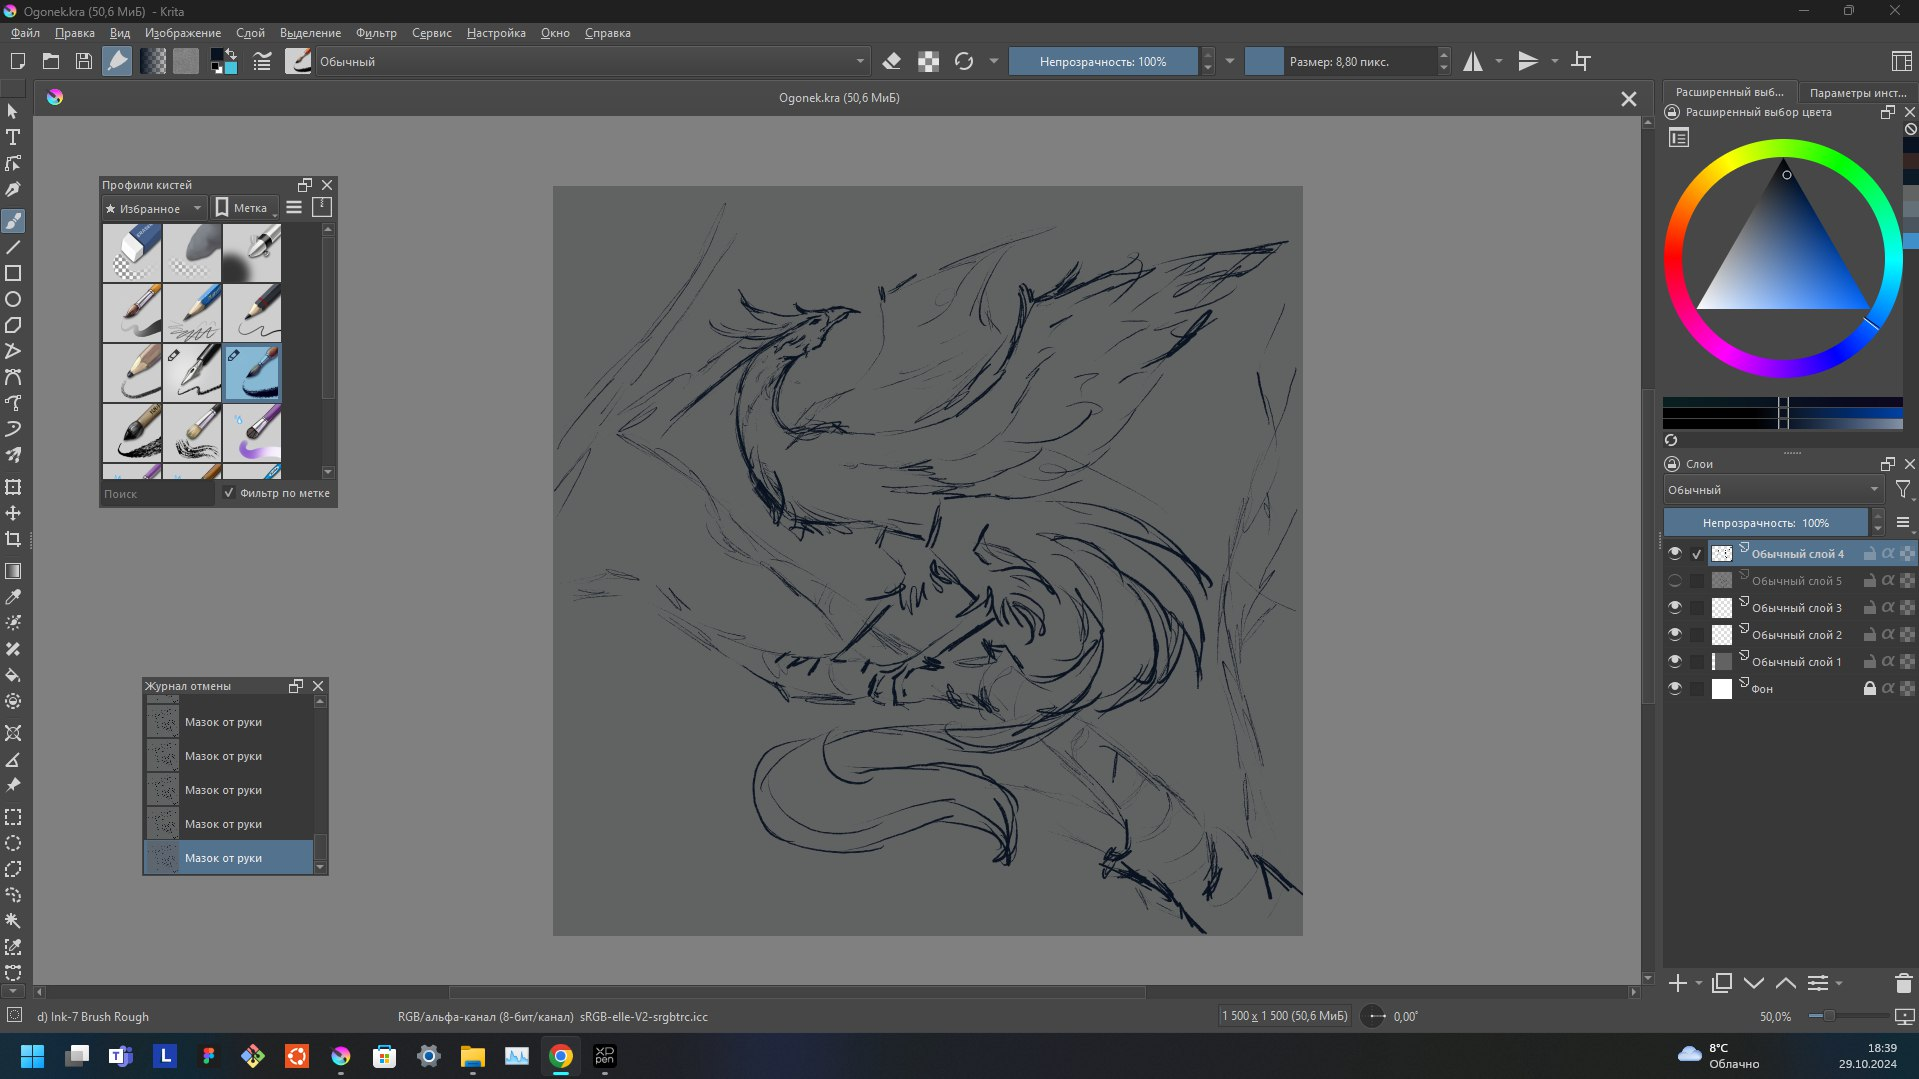
\includegraphics[width=0.50\linewidth]{Pictures/429b39b3-0e5e-4c1a-8a76-12356a091a6b.jpg}
    \caption{Самый первый набросок портрета}
    \label{fig:first}
    \end{figure}

    \begin{figure} [H]
        \centering
    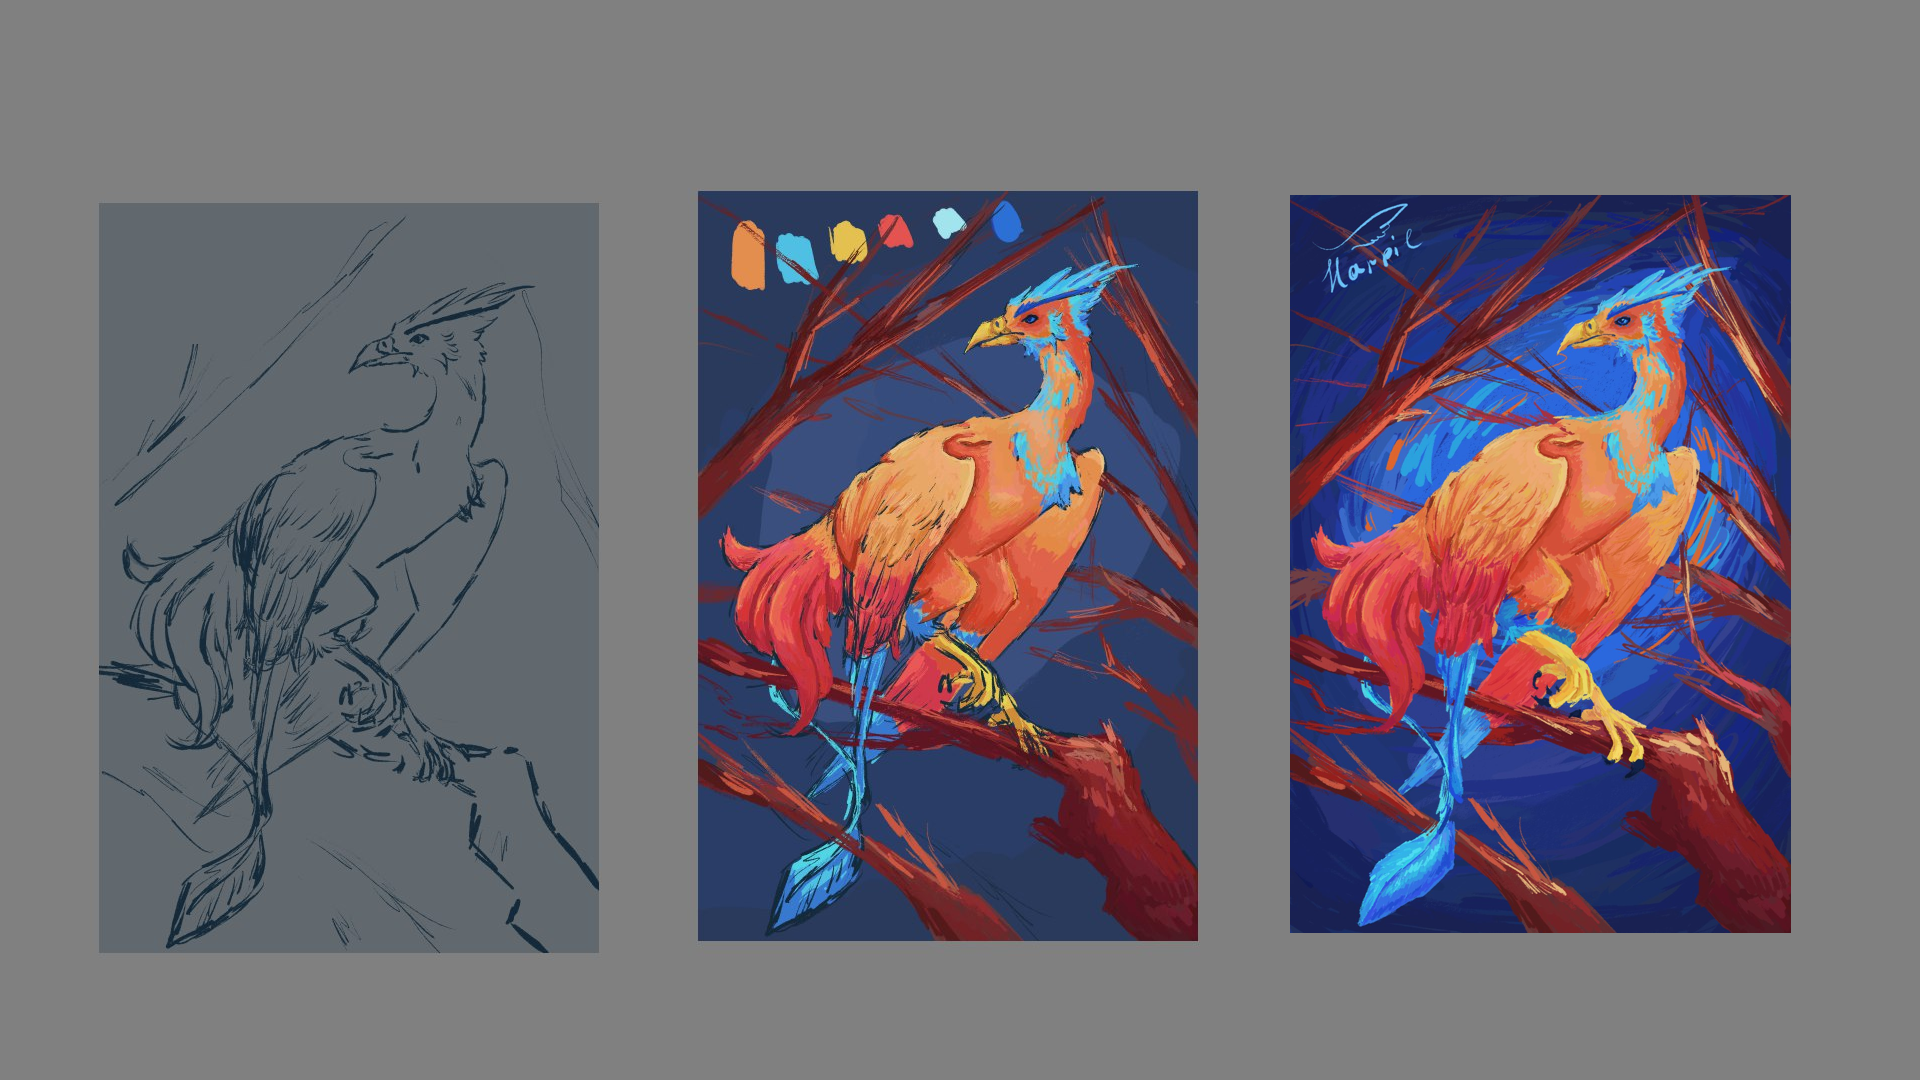
\includegraphics[width=0.50\linewidth]{Pictures/Procces.png}
    \caption{Этапы рисования портрета}
    \label{fig:process}
    \end{figure}

     \begin{figure} [H]
        \centering
    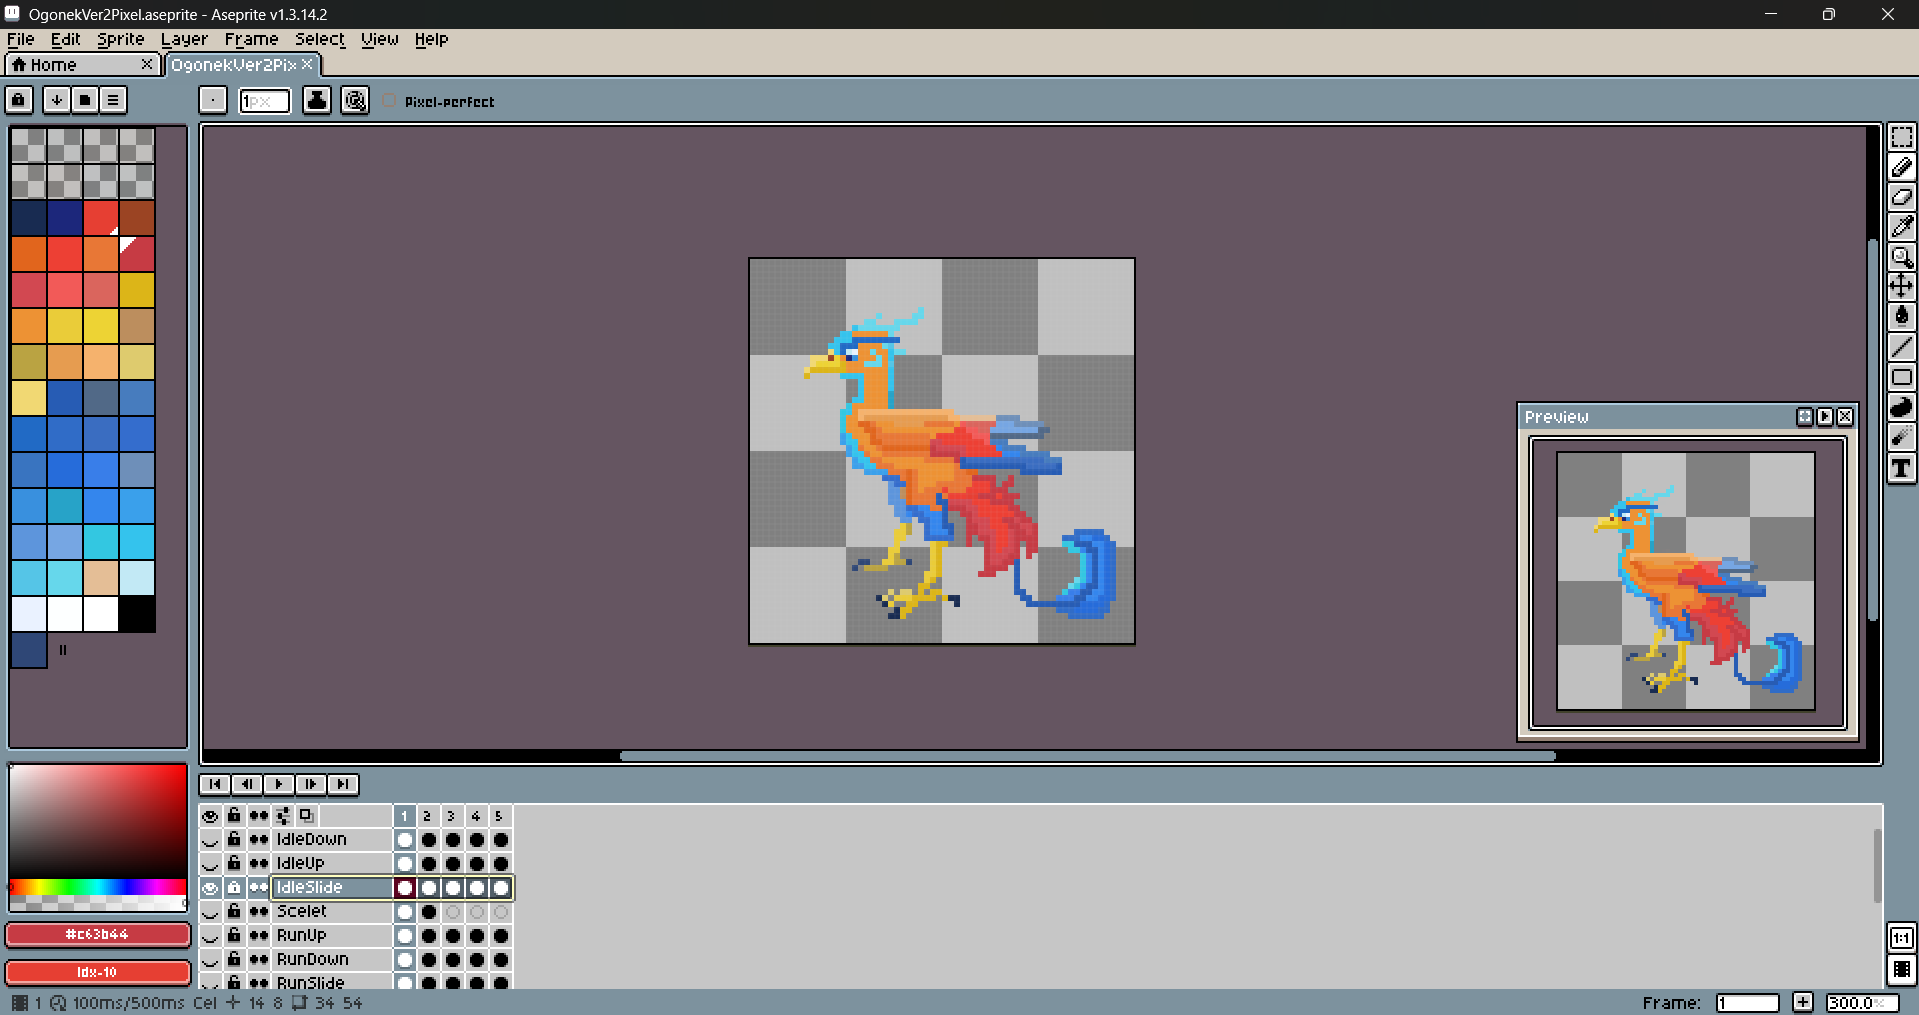
\includegraphics[width=0.50\linewidth]{Pictures/Снимок экрана 2025-06-24 162217.png}
    \caption{Самый первый спрайт}
    \label{fig:Acep}
    \end{figure}

    После было создано небольшое окружение для тестирования механик. 

     \begin{figure} [H]
        \centering
    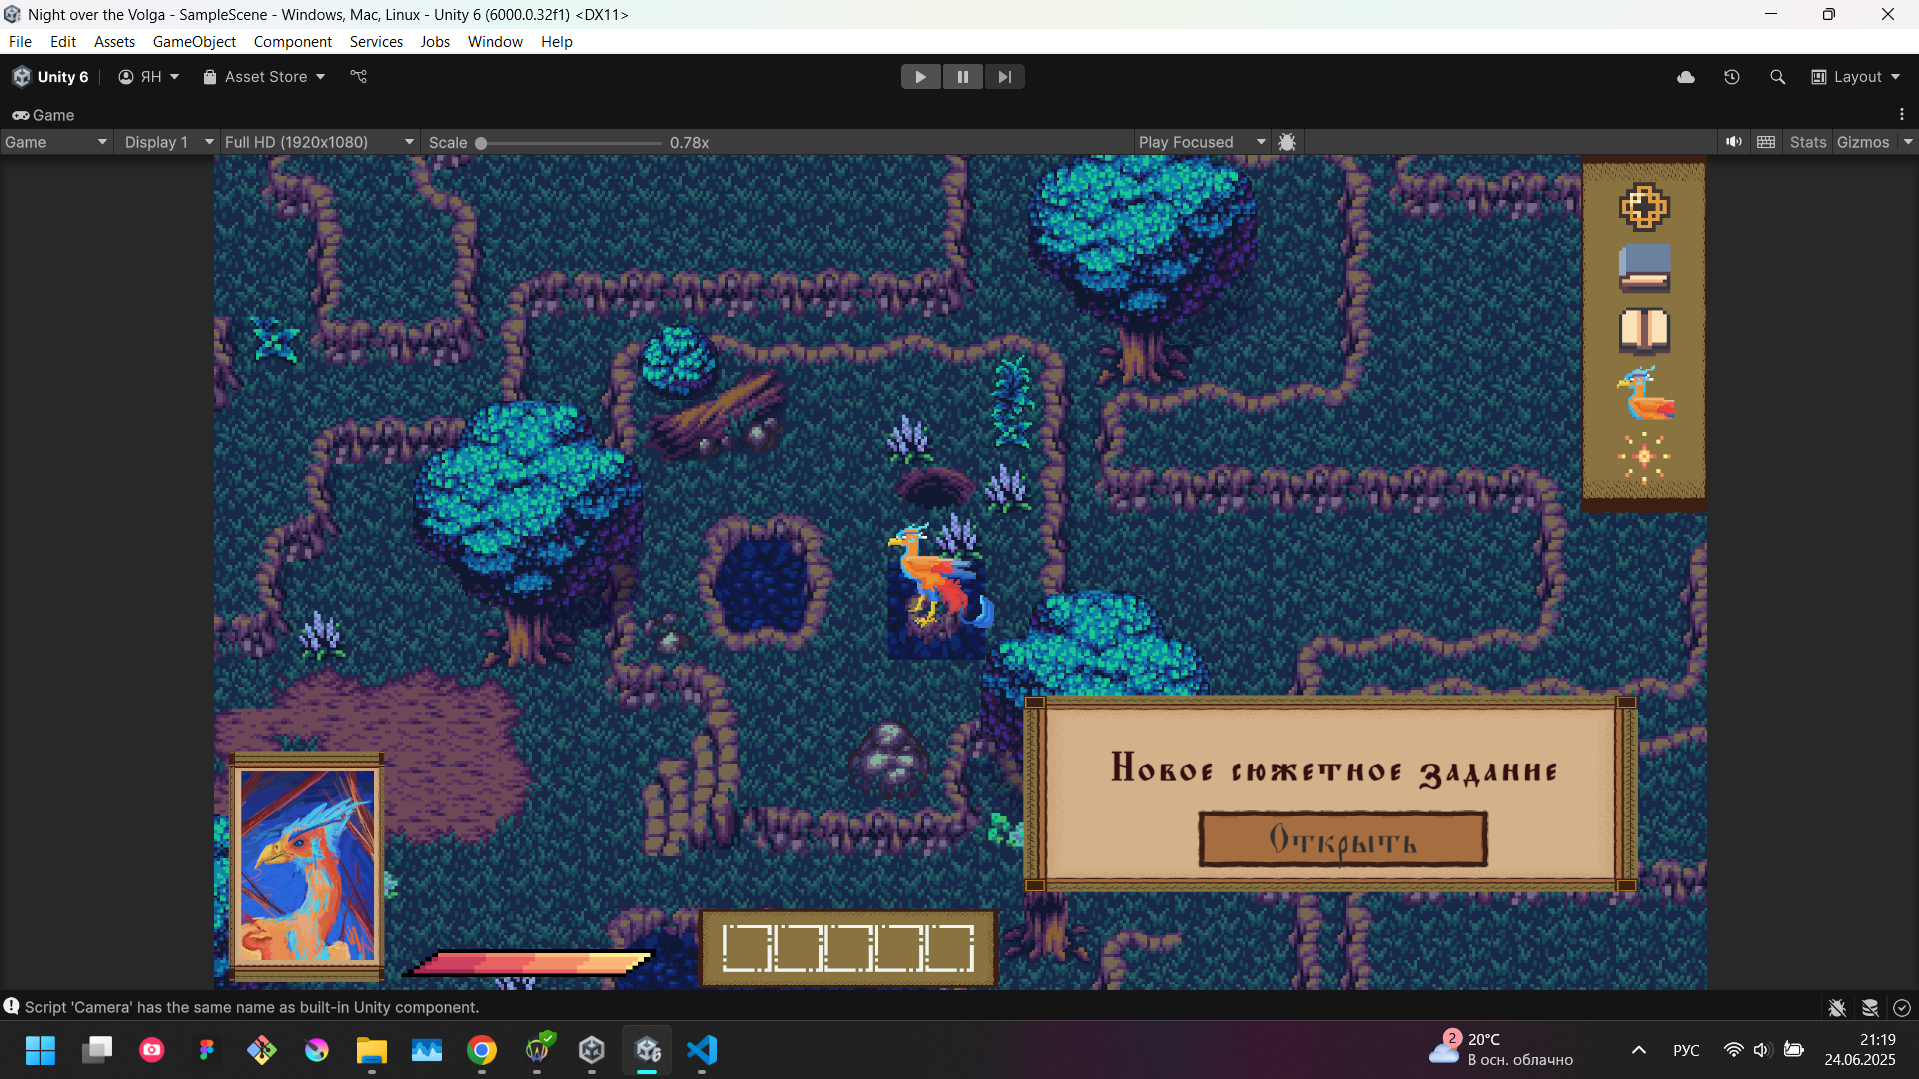
\includegraphics[width=0.50\linewidth]{Pictures/Снимок экрана 2025-06-24 211929.png}
    \caption{Тестовый вариант локации}
    \label{fig:Beginning}
    \end{figure}

    Как только было реализовано управление по нажатию кнопок, были добавлены 
    анимации для передвижения.

    \begin{figure} [H]
        \centering
    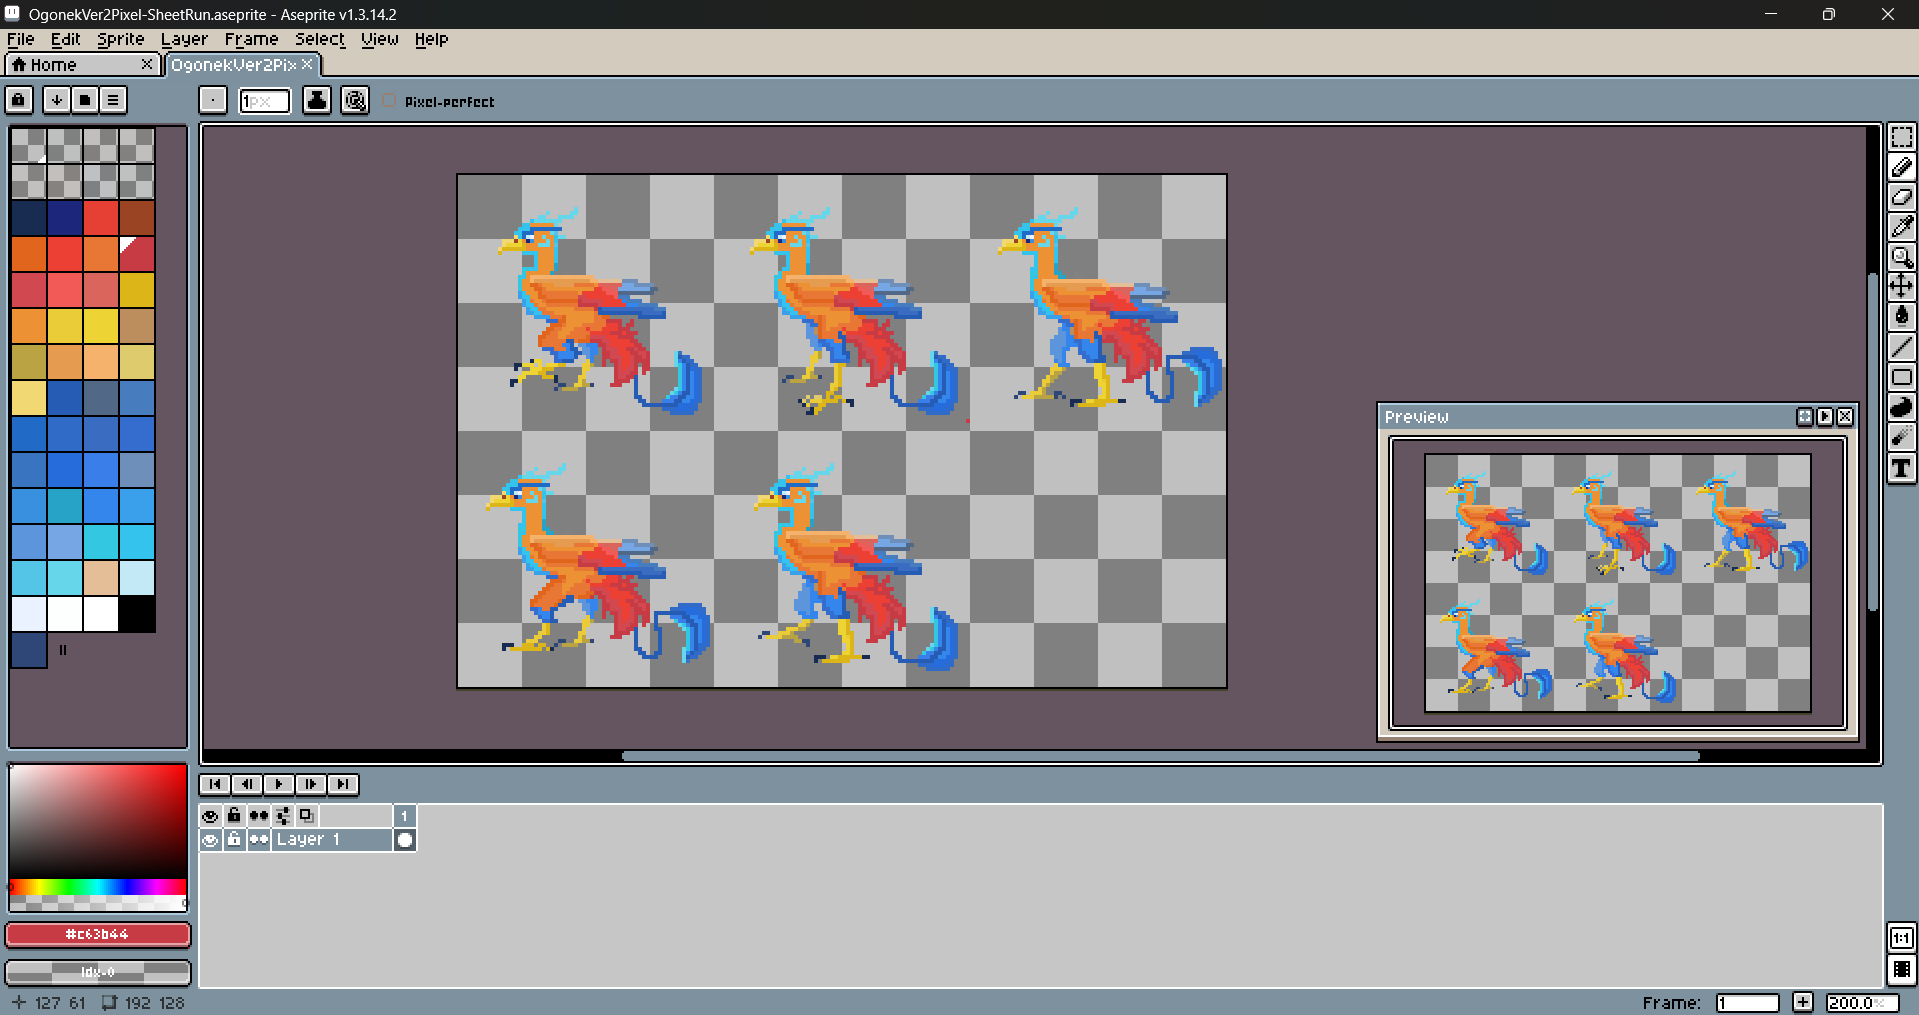
\includegraphics[width=0.50\linewidth]{Pictures/Снимок экрана 2025-06-24 162629.png}
    \caption{Кадры анимации бега}
    \label{fig:Run}
    \end{figure}
    
    Далее был создан интерфейс и реализован его функционал. 

    На карту были добавлены предметы для взаимодействия. 
    
    Последними этапами стали: добавления задания, врагов и выход из локации.

    Более подробно каждый аспект будет рассмотрен в каждом из разделов.

    \subsection{Общий алгоритм функционирования}

    При запуске игры первым, что видит пользователь это 
    главное меню где есть кнопки "Играть" и "Выход"(см. рисунок \ref{fig:MainMenu}). При нажатии на первую кнопку
    произойдет загрузка первой сцены - картинка с предысторией и кнопкой "Продолжить"
    (см. рисунок \ref{fig:Descript}),
     которая
    в свою очередь уже загрузит первую локацию. 
    А на вторую выход из игры соответственно. 

     \begin{figure} [H]
        \centering
    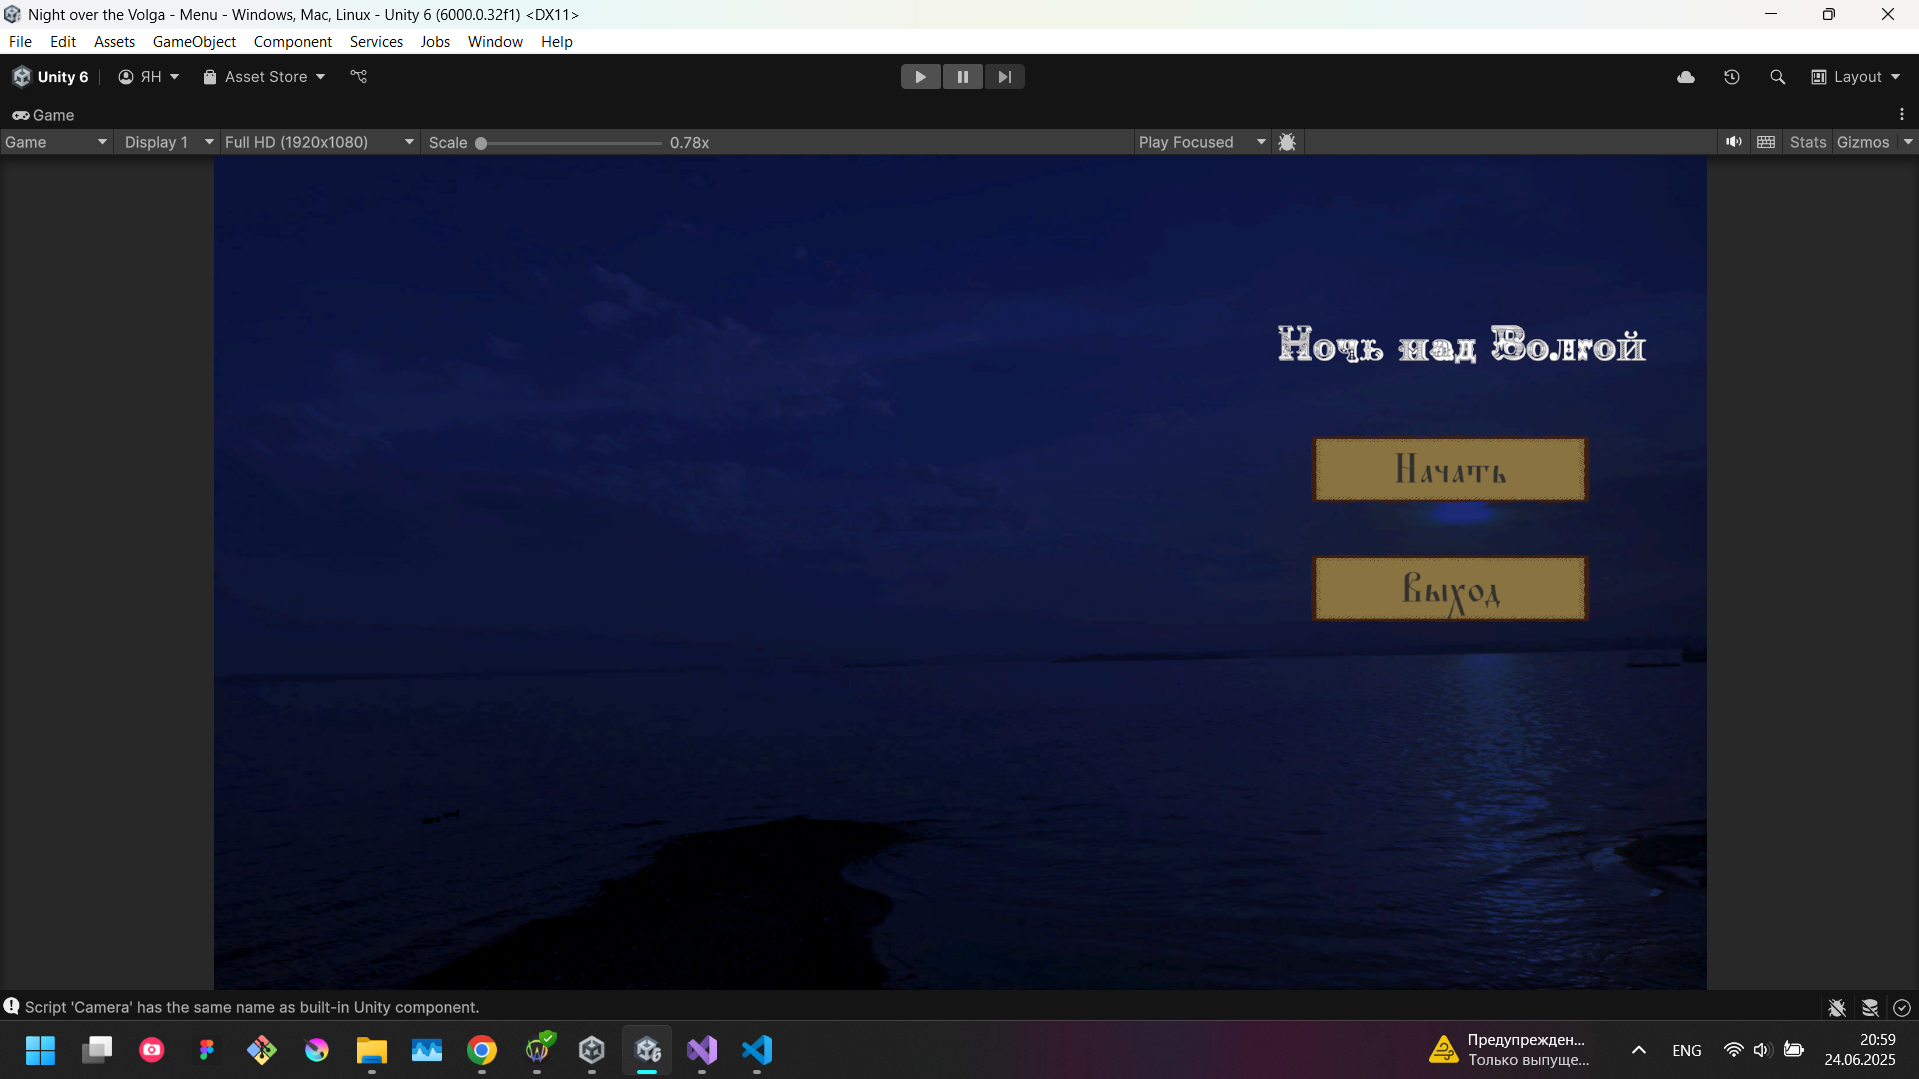
\includegraphics[width=0.50\linewidth]{Pictures/Снимок экрана 2025-06-24 205928.png}
    \caption{Первоначальное меню с альтернативным названием}
    \label{fig:MainMenu}
    \end{figure}


       \begin{figure} [H]
        \centering
    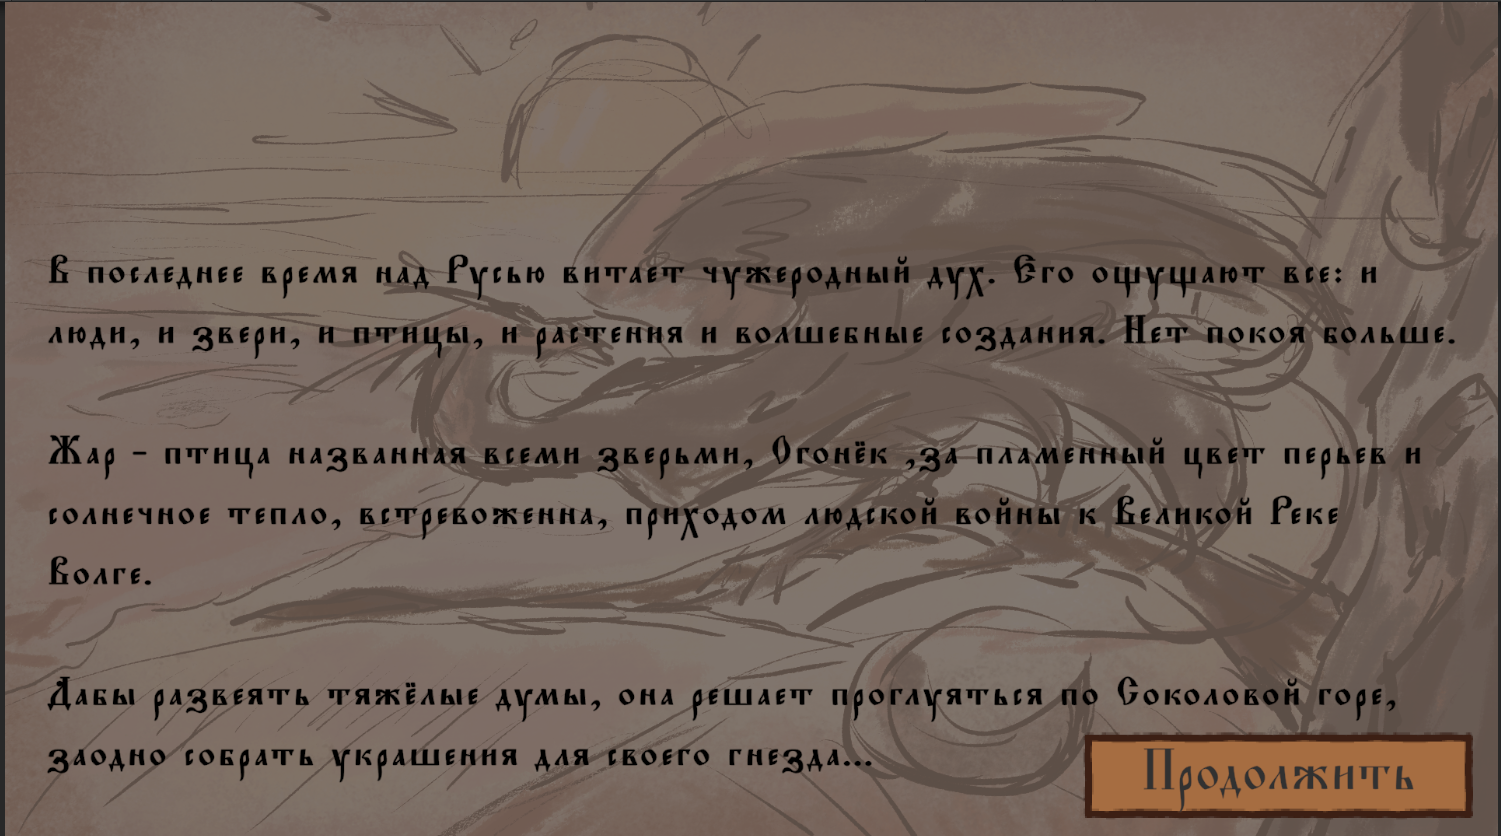
\includegraphics[width=0.50\linewidth]{Pictures/Снимок экрана 2025-06-24 211041.png}
    \caption{Текст с пояснением}
    \label{fig:Descript}
    \end{figure}


    Загрузка локаций происходит с помощью очереди сцен, которая задается 
    самим разработчиком(см. рисунок \ref{fig:Scene}).
    
     \begin{figure} [H]
        \centering
    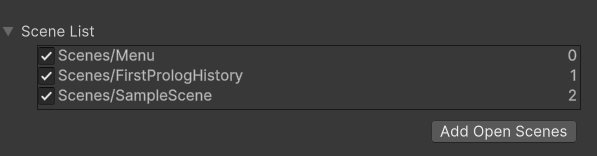
\includegraphics[width=0.50\linewidth]{Pictures/Снимок экрана 2025-06-24 203012.png}
    \caption{Очередь сцен}
    \label{fig:Scene}
    \end{figure}
    
    
    Очередь сцен представлена в самом Unity, но загрузка
    осуществляется с помощью кода. Ниже представлен код из файла "MainMeun.cs"
    \verbatiminput {Code/MainMeun.cs}

    После двух окон перед игроком предстает первая локация с главным героем, вернее
    героиней - жар-птицей, зовут которую Огонёк, о которой можно было немного узнать из небольшого пояснения в начале и окно с предложением,
    принять основное задание из длинной цепочки заданий (в данной курсовой реализована лишь самая малая её часть),
     завершив которую игра будет пройдена. 

     \begin{figure} [H]
        \centering
    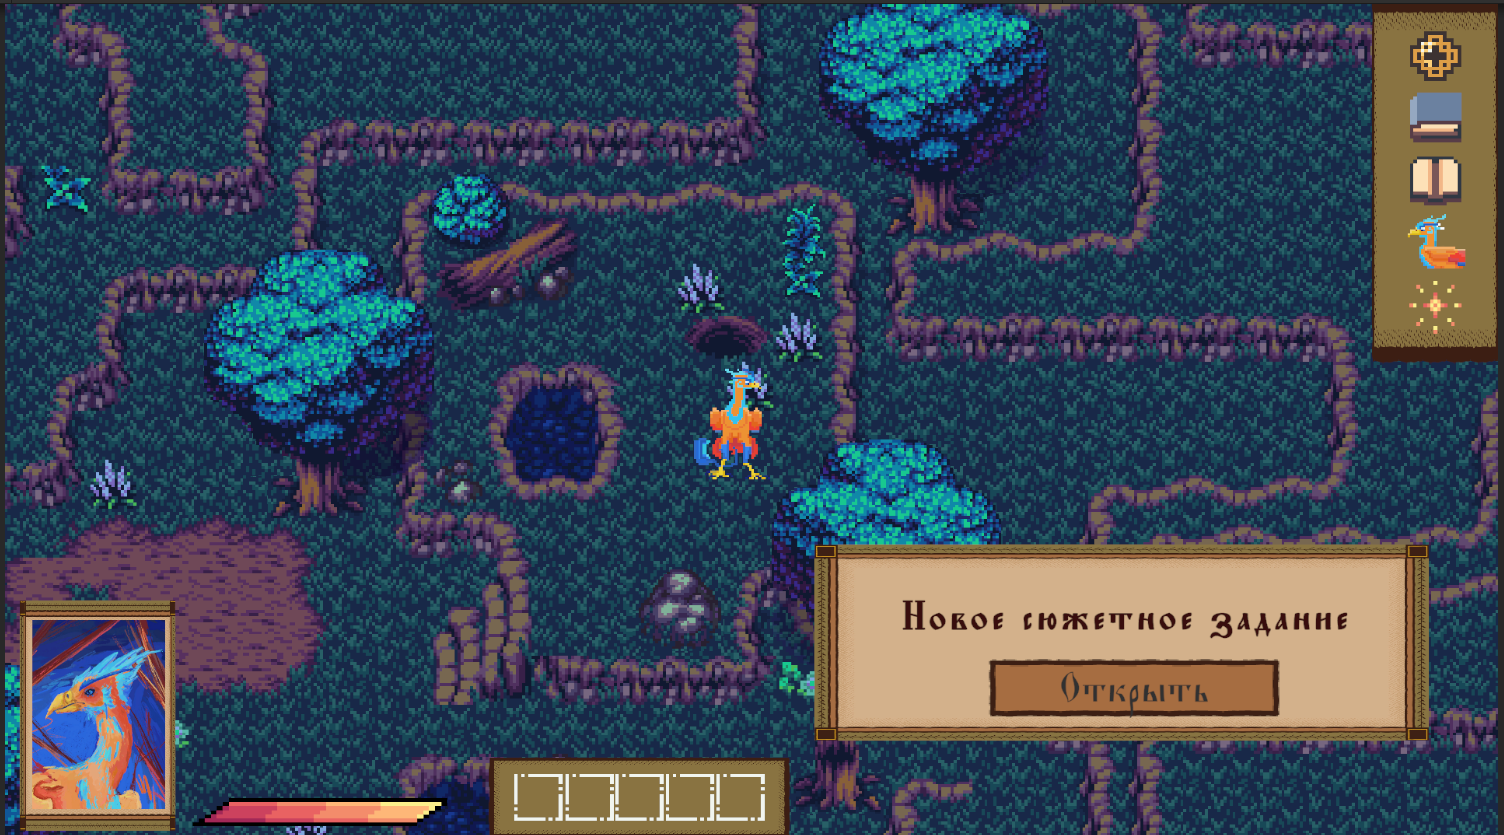
\includegraphics[width=0.50\linewidth]{Pictures/Снимок экрана 2025-06-24 212326.png}
    \caption{Начало игры}
    \label{fig:BeginningGame}
    \end{figure}

    После нажатия кнопки "Принять"(см. рисунок \ref{fig:Quest}), будет открыто окно с описанием задания, выполнив требования
    задания, его названием и наградой(в этом задание игрок получит 100 единиц опыта, которого по факту нет,
     т.к в рамках этой курсовой работы отсутствует развитие и персонажа и получение навыков) 
     игрок сможет перейти на вторую локацию, последнюю в прологе. 
    После принятия, на персонажа будет повешен маркер активного задания(см. рисунок \ref{fig:QuestFlag}). 


    \begin{figure} [H]
        \centering
    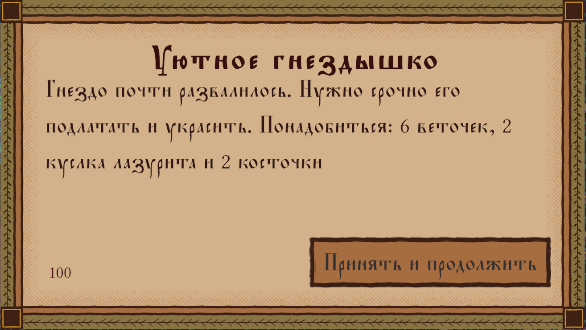
\includegraphics[width=0.50\linewidth]{Pictures/Снимок экрана 2025-06-24 212841.png}
    \caption{Окно принятия задания. От сюжетных заданий нельзя отказываться}
    \label{fig:Quest}
    \end{figure}


      \begin{figure} [H]
        \centering
    
\includegraphics[width=0.50\linewidth]{Pictures/Снимок экрана 2025-06-24 213521.png}
    \caption{Флаг активного задания, реализован с помощью булевой переменной}
    \label{fig:QuestFlag}
    \end{figure}

    Для передвижения используется стандартная раскладка - W,A,S,D. Скорость бега
    задается с помощью переменной типа int, а ее значение уже в инспекторе движка.
    Более подробно с кодом можно ознакомиться будет в папке с полной версией проекта на
    flash-накопителе. Анимация происходит благодаря внутреннему компоненту Unity - Animator
    (см. рисунок \ref{fig:Anim}).
    


 \begin{figure} [H]
        \centering
    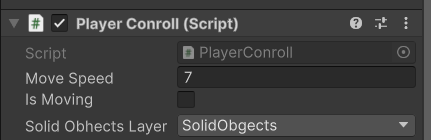
\includegraphics[width=0.50\linewidth]{Pictures/Снимок экрана 2025-06-24 214047.png}
    \caption{Часть инспектора}
    \label{fig:Move}
    \end{figure}


     \begin{figure} [H]
        \centering
    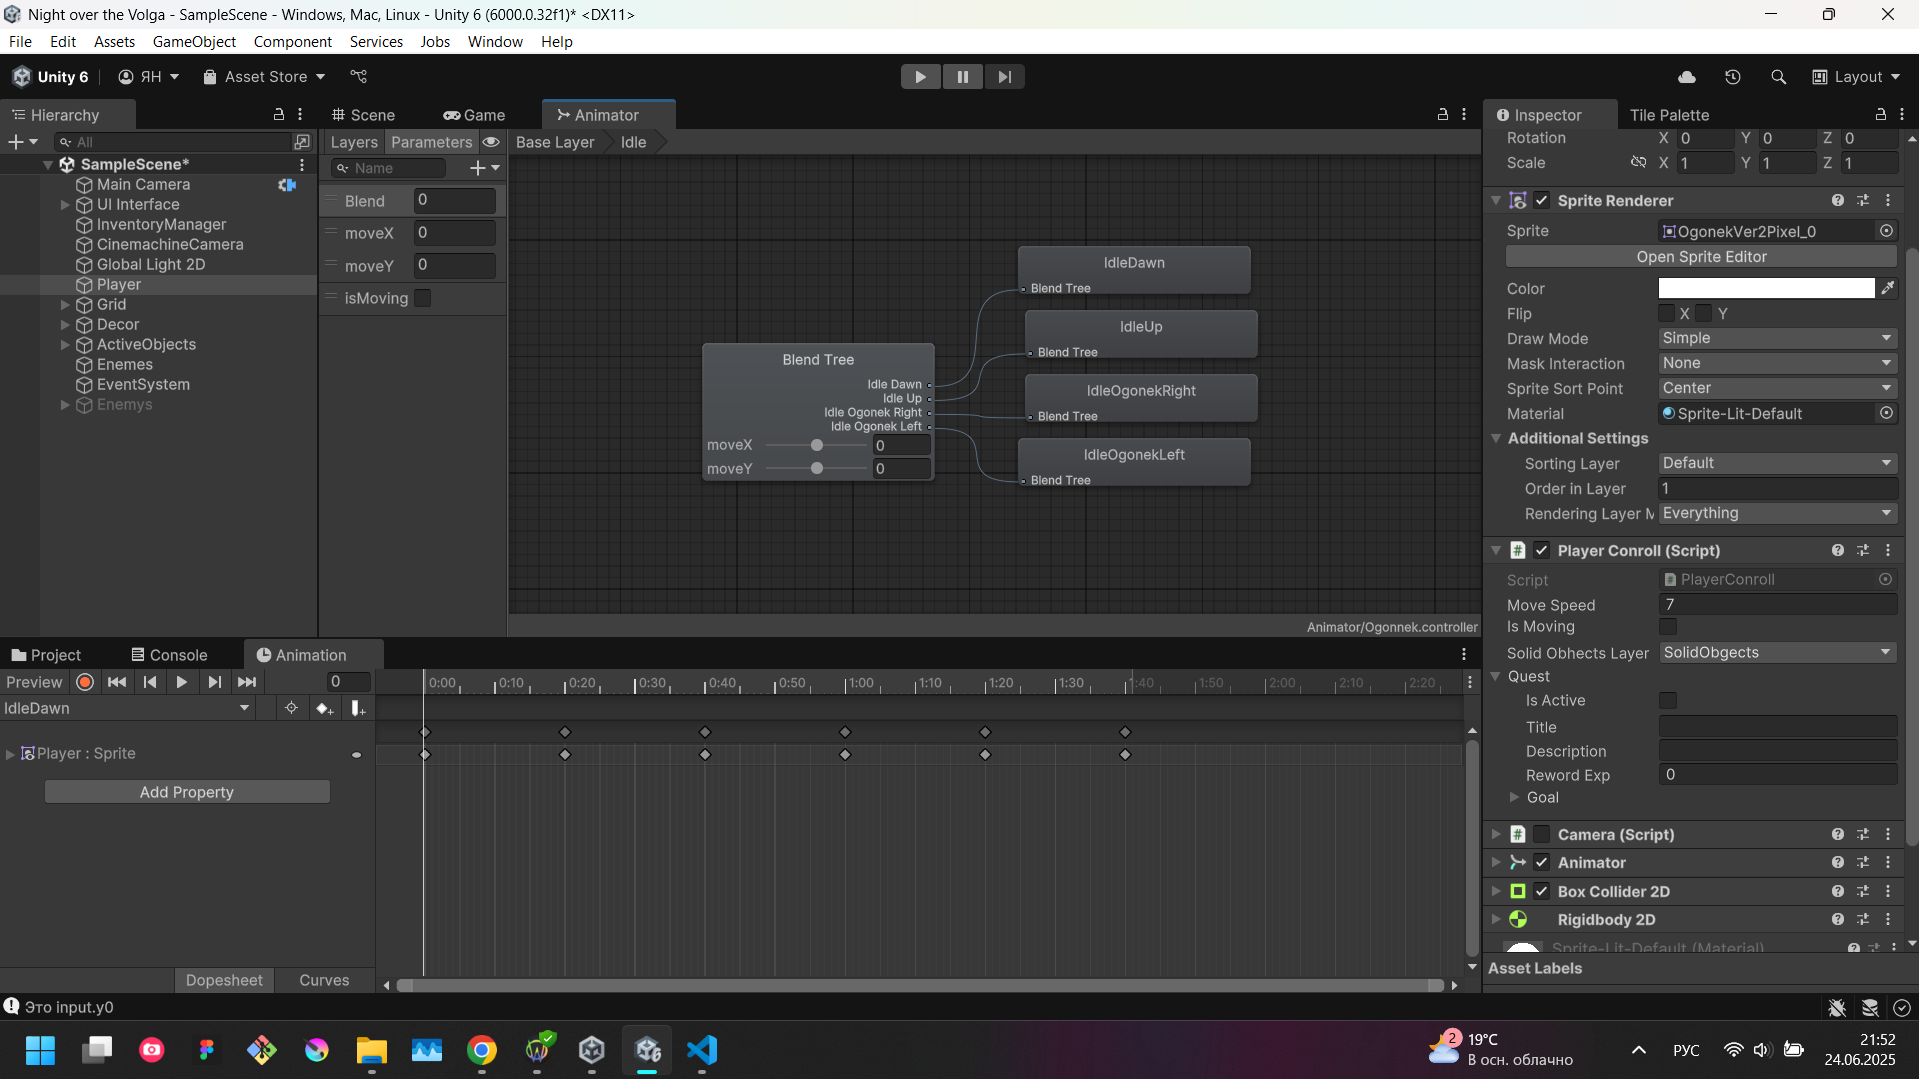
\includegraphics[width=0.50\linewidth]{Pictures/Снимок экрана 2025-06-24 215301.png}
    \caption{Окно аниматора и анимаций}
    \label{fig:Anim}
    \end{figure}

    Атака же осуществляется на нажатие ПКМ, нажав ее персонаж выпустит "Огненный Всплеск" - 
    базовая атака дальнего боя.


    \begin{figure} [H]
        \centering
    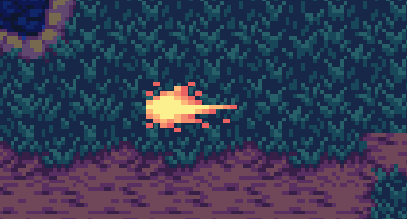
\includegraphics[width=0.50\linewidth]{Pictures/Снимок экрана 2025-06-24 220136.png}
    \caption{Спрайт атаки}
    \label{fig:Anim}
    \end{figure}

    Как было представлено на рисунке \ref{fig:Descript}, целью задания найти материалы,
    при прикосновение персонажа к предмету, он попадает в инвентарь и исчезает с локации.
    Если конечно же есть место в инвентаре, в противном случае объект останется на своем месте.

    Код отвечающий за подбор предметов представлен ниже:
    С полным кодом отвечающим за функционирования инвентаря можно ознакомиться в приложение А.
    \begin{verbatim}
         public void Pickupitem(int id)
    {
        bool result=inventoryManager.AddItem(itemsToPickUp[id]);
        if (result is true)
        {
            Debug.Log("Да");
        }
        else
        {
            Debug.Log("Нет");

        }
    }
    \end{verbatim}

    \begin{figure} [H]
        \centering
    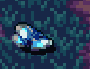
\includegraphics[width=0.50\linewidth]{Pictures/Снимок экрана 2025-06-24 220509.png}
    \caption{Лазурит - один из материалов}
    \label{fig:Lazurit}
    \end{figure}
        
    \subsection{Создание игровых классов и объектов}

    Самым первым объектом создавался "Player". Это один из главных объектов в проекте.
    В начале в окне иерархии создается пустой Game Object, затем к объекту прикрепляются компоненты, их можно 
    увидеть на рисунке \ref{fig:Comp}

     \begin{figure} [H]
        \centering
    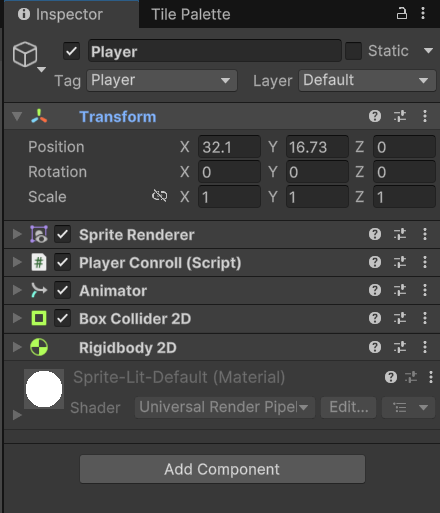
\includegraphics[width=0.50\linewidth]{Pictures/Снимок экрана 2025-06-24 222030.png}
    \caption{Компоненты}
    \label{fig:Comp}
    \end{figure}

    Transform - отвечает за позицию, поворот и масштабирование объекта.

    Player Conroll (Script) - код отвечающий за поведение персонажа.

    Animator - Содержит анимации и их порядок воспроизведения.

    Box Collider 2D - форма, определяющая форму объекта для целей физических столкновений.

    Rigidbody 2D - объект становиться физическим телом и имеет свою физику, которую можно
    при желании более детально настроить.

    Часть кода для управление персонажем представлена ниже:
    

    \begin{verbatim}

           private void Awake()
    {
        ogonekanimator= GetComponent<Animator>();
    }



    private void Update()
    {

        if (!IsMoving)
        {
            input.x = Input.GetAxisRaw("Horizontal");
            input.y = Input.GetAxisRaw("Vertical");

            Debug.Log("Это input.x" + input.x);
            Debug.Log("Это input.y" + input.y);

            if (input.x != 0) input.y = 0; 

            if (input !=Vector2.zero) 
            {
                ogonekanimator.SetFloat("moveX", input.x);
                ogonekanimator.SetFloat("moveY", input.y);
              
                var TargetPos = transform.position;
                TargetPos.x += input.x;
                TargetPos.y += input.y;

                if(IsWallcable(TargetPos)) 
                StartCoroutine(Move(TargetPos));

            }
        }

        ogonekanimator.SetBool("isMoving", IsMoving);
    }

    IEnumerator Move (Vector3 TargetPos)
    {
        IsMoving= true;

        while((TargetPos- transform.position).sqrMagnitude > Mathf.Epsilon) 
        {
            transform.position = Vector3.MoveTowards(transform.position, TargetPos, 
            MoveSpeed * Time.deltaTime);
            yield return null;
        
        }
        transform.position = TargetPos;
        IsMoving= false;

    }

    private bool IsWallcable(Vector3 TargetPos)
    {
        if(Physics2D.OverlapCircle(TargetPos, 0.1f, solidObhectsLayer) != null)
        {
            return false;
        }
        return true;

    }

    \end{verbatim}

    С интерфейсом похожая ситуация. Начало тоже самое, но в отличие от "Player", используется
    не пустой Game Object, а специальный - Canvas. Создается родительский объект 
    "UI interface" от которого будет зависеть интерфейс, к нему крепиться файл "WindowManager.cs", 
    собственно  он отвечает за корректную работу окон.


    \begin{verbatim}
        public class WindowManager : MonoBehaviour 
{
    public static WindowManager Instance { get; private set; }

    private MenuWindow _lastActiveWindows;

    public bool HaveOpenWindow => _lastActiveWindows is not null;



    public void Awake()
    {
        Instance = this;
    }

    public void Open(MenuWindow menuWindow)
    {
        if(_lastActiveWindows == menuWindow)
        {
            Close();
            return;
        }
        else if (_lastActiveWindows is not null)
        {
            _lastActiveWindows.Close();
        }

        _lastActiveWindows = menuWindow;
        menuWindow.Open();
    }

    public void Close()
    {
        if(_lastActiveWindows is not null)
        {
            _lastActiveWindows.Close();
            _lastActiveWindows = null;
        }
    }
}
    \end{verbatim}

    Более подробно создание интерфейсов, будет рассмотрено в подпункте 2.5. 
    
    \subsection{Создание 2D модели персонажа}

    В самом начале создаются несколько набросков персонажа. Они представляют идеи как
    примерно будет выглядеть персонаж. После отбирается наиболее удачный, начинается проработка деталей.
    После этого этапа выбираются выбираются базовые цвета. Иногда на этом этапе облик персонажа
    может притереть изменения, как видно на рисунках \ref{fig:first} и \ref{fig:process}, приведенных
    выше в разделе 2.
    
    Спрайт тоже претерпел изменения из-за изменения портрета. 

     \begin{figure} [H]
        \centering
    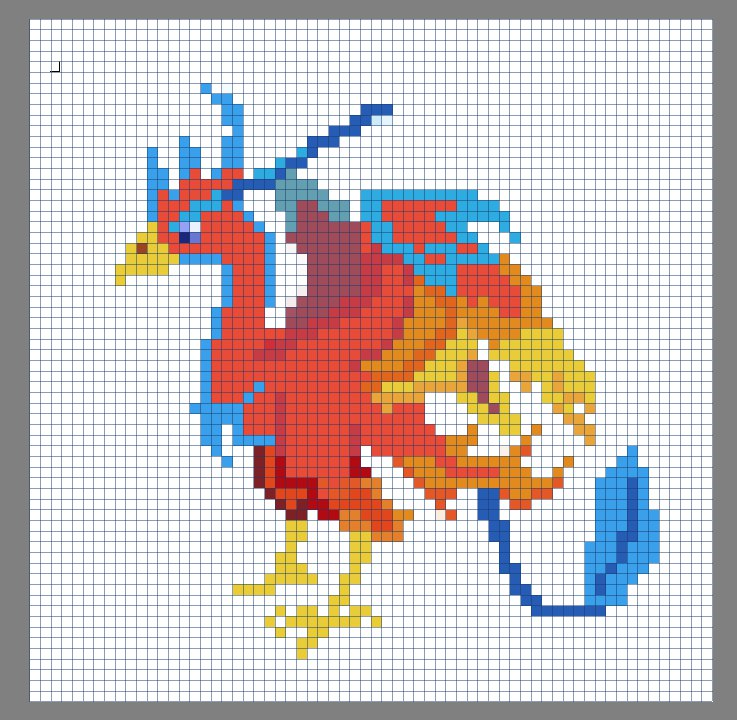
\includegraphics[width=0.35\linewidth]{Pictures/ab7b4ae0-60bd-4de1-af7b-8cec77c285f7.jpg}
    \caption{Самый первый спрайт}
    \label{fig:firstSprite}
    \end{figure}

     \begin{figure} [H]
        \centering
    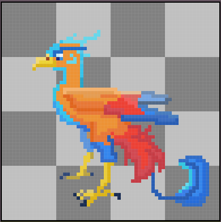
\includegraphics[width=0.35\linewidth]{Pictures/Снимок экрана 2025-06-25 195944.png}
    \caption{Финальный вариант}
    \label{fig:firstSprite}
    \end{figure}

    После того как был утвержден финальный вариант. Делаются кадры анимации.
    Так как игра изометрическая, то пришлось делать анимации для трех позиций: влево-вправо(происходит
    отзеркаливание) лицом к игроку и спиной к игроку. 

     \begin{figure} [H]
        \centering
    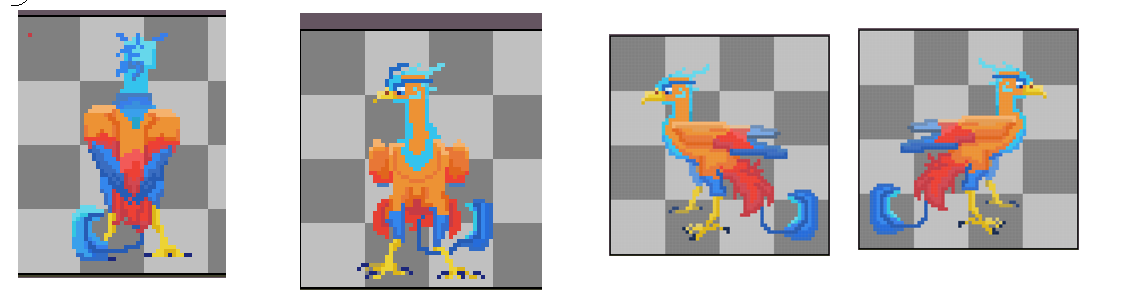
\includegraphics[width=0.50\linewidth]{Pictures/Снимок экрана 2025-06-25 201224.png}
    \caption{Птица с разных сторон}
    \label{fig:Sprites}
    \end{figure}



    \subsection{Создание уровней}

    Создание уровней в Unity происходит с помощью так называемых сцен. Сцены содержат объекты игры,
    причем они могут использоваться как для создания меню, так и отдельных уровней.

    Что бы создать уровень, нужно в начале создать Tile Palette. Для этого нужно создать текстуры 
    окружение мира,
    т.е нарисовать их, либо использовать из бесплатных открытых асетов. Поседений вариант был выбран.
    После этого нужно импортировать асет в Unity, когда он будет внутри движка, нужно 
    открыть окно Tile Palette и в диалогом окне выбрать "New Palette", а после "Create New Palette".
    После нужно перенести текстуры в "Tile Palette" и нажать на кнопку сохранить, затем выбрать куда
    нужно сохранить Tile Asset\cite{search5}. 

    Когда все будет сделано, можно будет "рисовать" получившимися текстурами. Когда окружение будет 
    закончено, где есть текстуры объектов(например камней), надо добавить коллайдеры.
    Что бы игрок не проходил сквозь текстуры. 

    \begin{figure} [H]
        \centering
    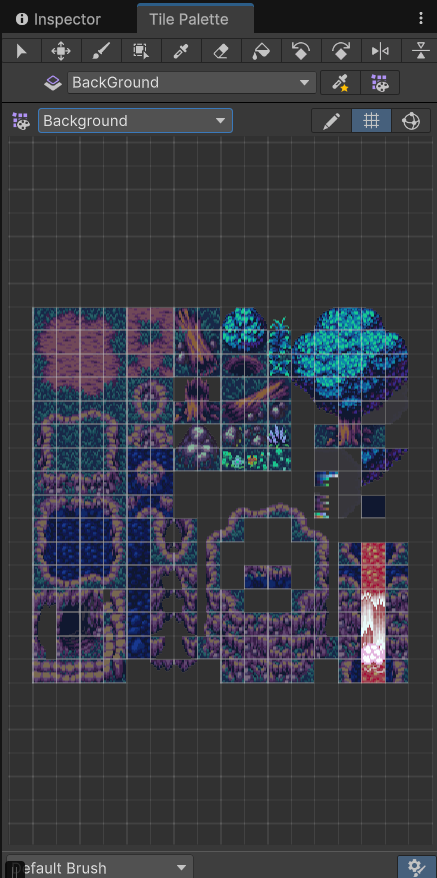
\includegraphics[width=0.50\linewidth]{Pictures/Снимок экрана 2025-06-25 203428.png}
    \caption{Окно Tile Palette с текстурами}
    \label{fig:Textures}
    \end{figure}

    Существует множество способов создания коллайдеров. Один из них создать новый "Tile Palette",
    с одним белым спрайтом. Назвать его к примеру "Solid". Но перед этим из белого спрайта сделать 
    так называемый prefab и добавить ему компонент Collider 2D. 
    После как и с обычными текстурами "красить" им нужные места.

    \begin{figure} [H]
        \centering
    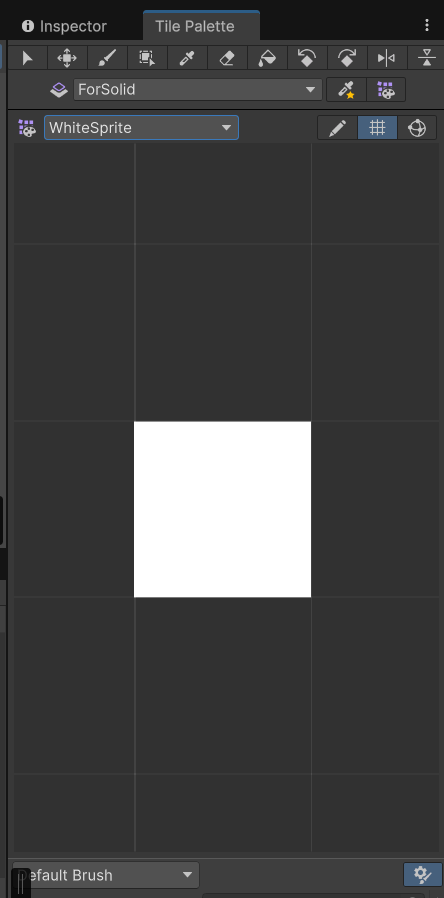
\includegraphics[width=0.50\linewidth]{Pictures/Снимок экрана 2025-06-25 203441.png}
    \caption{Окно Tile Palette с белым спрайтом}
    \label{fig:Textures}
    \end{figure}

    Когда процесс будет завершен, нужно сделать спрайт прозрачным. Этот способ хорош тем, что
    нагрузка на движок и на компьютер снижается, благодаря чему приложение будет быстрее работать.

    Когда уровень готов на него добавляются объекты и скрипты.

    После чего идет тестирование на проверку "плотности" текстур, чтобы игрок случайно не 
    прошел сквозь объект или стену. В конце проверяются предметы, тестировщик смотрит
    исчезают они при каких либо условиях, или как то ещё "странно себя ведут", особенно, если
    они заскриптованы.
    Наконец наступает очередь скриптов. Тестировщик всячески пытается выявить "брешь" в них,
    сломать их. Иными словами проверяет их на "прочность". Это делается, чтобы понять,
    какие действия игрока могут сломать логику, к примеру тех же заданий, из-за чего оно 
    может стать не выполнимым.
   
    \subsection{Создание интерфейсов}

    Интерфейс в Unity создается с помощью компонента "Canvas"\cite{search6}. Сам Canvas представляет 
    собой абстрактное пространство, 
    в котором производится настройка и отрисовка UI.

    В начале создается родительский объект "UI interface". К нему крепиться весь интерфейс.
    Это сделано для того что бы каждый раз не задавать настройки окнам. Так 
    все дочерние объекты, которыми являются окна, а также другие
    компоненты интерфейса, к примеру панель меню, будут наследовать
    параметры главного родительского объекта.


     \begin{figure} [H]
        \centering
    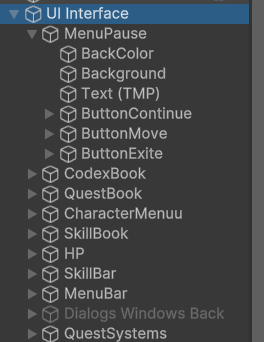
\includegraphics[width=0.50\linewidth]{Pictures/Снимок экрана 2025-06-25 205359.png}
    \caption{Иерархия интерфейса}
    \label{fig:Textures}
    \end{figure}

    Так же к каждому дочернему объекту крепятся нужные компоненты. К примеру код.
    Каждое окно имеет свой код с соответствущим функционалом. Подробно с ним можно
    ознакомиться в папке с исходным кодом "Scripts" на flash-накопителе.
    Ниже приведен пример кода из файла MenuBar.cs отвечающий за панель меню:
    
    \verbatiminput {Code/MenuBar.cs}


    \subsection{Тестирование игры}

    Тестирование игры происходило в несколько этапов.

    Самым первым этапом стало так называемое "модульное тестирование"\cite{test}.
    Это проверка на корректность работы отдельных компонентов игры отдельно друг от друга.

    Для примера можно взять кнопки кодекса, при нажатии раскрывается текст(см. рисунки 
    \ref{fig:TextClose} и \ref{fig:TextOpen}).

 \begin{figure} [H]
        \centering
    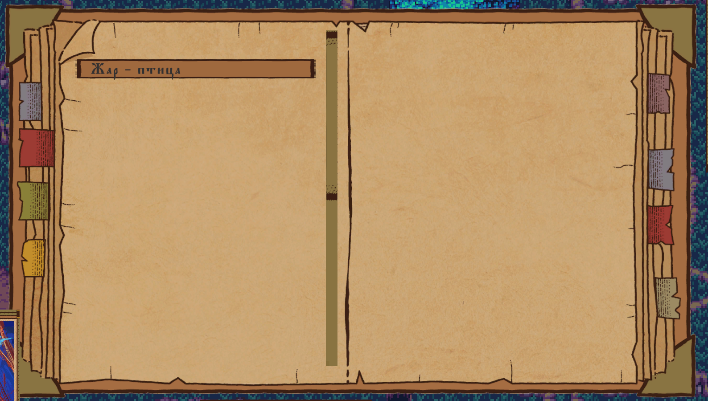
\includegraphics[width=0.50\linewidth]{Pictures/Снимок экрана 2025-06-25 212028.png}
    \caption{Текст по умолчанию скрыт}
    \label{fig:TextClose}
    \end{figure}


 \begin{figure} [H]
        \centering
    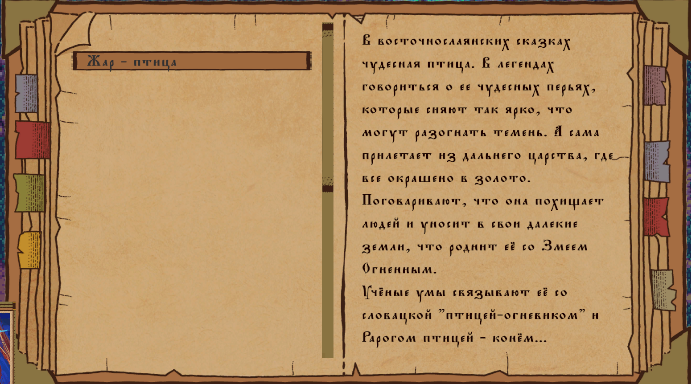
\includegraphics[width=0.50\linewidth]{Pictures/Снимок экрана 2025-06-25 212038.png}
    \caption{Раскрытый текст}
    \label{fig:TextOpen}
    \end{figure}

    
    Вторым же этапом стало интеграционное тестирование. Это нужно, чтобы проверить
    как взаимодействуют компоненты между собой.
    К примеру: проверялось добавление предметов в инвентарь, так как,
    когда инвентарь попадает в инвентарь, он не просто исчезает, а становиться "частью интерфейса".
    
    А когда открыто любое окно интерфейса, оно "замораживает" все процессы в игре.

    На этом основные этапы закончены. Далее идёт выявление критических ошибок, которые могут привести
    к вылету игры и прочему. Потом уже не значительных ошибок, одной из них стало 
    сообщение об отсутствии canvas, данная ошибка не приводит ни к чему кроме сообщения в
    логе движка, а так же к не самому плавному перетаскиванию объектов в инвентаре.
     По факту она видна только разработчику. 

     Так же одним из неприятных багов является прохождение текстур сквозь друг друга.

     \begin{figure} [H]
        \centering
    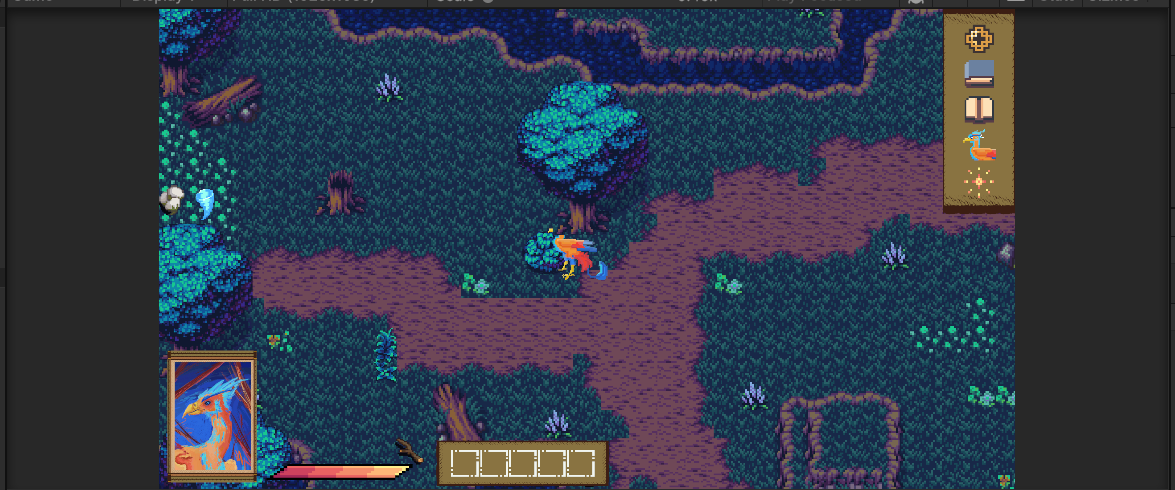
\includegraphics[width=0.50\linewidth]{Pictures/Снимок экрана 2025-06-25 213248.png}
    \caption{Текстуры персонажа проходят сквозь дерево и наслаиваются на куст}
    \label{fig:Bug}
    \end{figure}





% Раздел "Заключение"
\conclusion

   Процесс разработки игры – это сложный, многоэтапный и творческий процесс, 
   требующий не только технических навыков,
    но и художественного видения. 
    Несмотря на то, что современные игровые движки, 
    такие как Unity, значительно упрощают многие аспекты разработки – от работы с графикой и физикой 
    до управления анимацией и скриптами – создание качественной игры по-прежнему 
    остаётся трудоёмкой задачей. Разработчикам приходится продумывать геймдизайн, 
    баланс игровых механик, нарратив, уровень-дизайн, 
    звуковое сопровождение и оптимизацию под разные платформы.

    В ходе данной работы были успешно выполнены ключевые задачи, направленные на разработку базовых
    механик игры. Так же были изучены игровые движки, что позволило
    выбрать самый подходящий для эффективной разработки.
     В будущем проект можно будет доработать, что бы он стал полноценной игрой,
    которую можно будет выпустить на рынок.  



    \bibliographystyle{ugost2008.bst}
    \bibliography{thesis}
    
    \appendix

    \section{Полный код для работы инвентаря}
    \verbatiminput {Code/InvenoryManager.cs} 
    \verbatiminput {Code/InvenoryItem.cs}
    \verbatiminput {Code/InventorySlot.cs}
    \verbatiminput {Code/Loot.cs}

    \section{Flash-носитель с отчетом о выполненной работе}

    На приложенном flash-накопителе можно ознакомиться со следующими
файлами:

\begin{description}
\item[Папка \texttt{Course}] "---   \LaTeX- вариант курсовой работы;
\item[Папка \texttt{Scripts}] "--- весь исходный код игры;
\item[Папка \texttt{Night over the Volga}] "--- игра;

\item[\texttt{Course.pdf}] "--- курсовая работа.
\end{description}

    
\end{document}